\documentclass{article}
\usepackage{graphicx}
\usepackage[polish]{babel}
\usepackage[T1]{fontenc}
\usepackage{enumitem}
\usepackage{float}
\usepackage{hyperref}
\usepackage{amsmath}
\usepackage{booktabs}

\title{Analiza zależności kosztu komórki od parametrów symulacji w grze Cell Evolution}
\author{Mikołaj Kubś}
\date{Czerwiec 2024}

\begin{document}

\maketitle
\tableofcontents

\newpage

\section{Wstęp}
Poniższa praca będzie zajmować się badaniem zależności średniego kosztu komórki (average creature cost) w grze Cell Evolution od początkowych parametrów symulacji. Koszt komórki oznacza ilość energii, jaką organizm potrzebuje, by przeprowadzić mitozę ("koszt" genu/części ciała/akcji w raporcie będzie zawsze oznaczał koszt energetyczny - czyli jedzenie przetworzone na energię). Parametrami początkowymi będą:
\begin{itemize}[itemsep=0mm]
    \item wielkość mapy (map size),
    \item liczba początkowych komórek (starting creatures),
    \item okres czasu między powstaniem nowego jedzenia (time to spawn a food),
    \item mnożnik mutacji (mutation range),
    \item mnożnik prawdopodobieństwa mutacji części ciała (body part mutation chance),
    \item okres czasu między reprodukcją (interval between births),
    \item mnożnik wpływu wieku na głód (hunger mult from age),
    \item mnożnik agresywności (aggresivnes mult),
    \item mnożnik kosztu genów (genes cost mult),
    \item mnożnik kosztu części ciała (body parts cost mult).
\end{itemize}
Najpierw zostanie przeprowadzona regresja liniowa, by estymować koszt komórki z parametrów początkowych. Następnie sprawdzona będzie hipoteza, czy uwzględnienie w modelu innych danych końcowych (rezultatów) symulacji zwiększy jego jakość.

Dodatkowo zostaną utworzone trzy modele regresji, które będą ze sobą porównane po zoptymalizowaniu.

Pomysł projektu zainspirowany był chęcią sprawdzenia, czy w grze Cell Evolution dałoby się przewidzieć różne dane końcowe na podstawie parametrów symulacji. Oznaczałoby to, że różne symulacje o tych samych parametrach kończyłyby się podobnym skutkiem. W grze występuje jednak dużo losowości - jedzenie powstaje w różnych miejscach, agenci przy polowaniu wybierają swoje ofiary niederministycznie, mutacje odbywają się losowo i wiele więcej. 

\section{Opis działania symulacji w Cell Evolution}
W tej grze, na podstawie parametrów początkowych, tworzona jest mapa wraz z początkową populacją, której wartości wszystkich genów są bliskie 0,5. Następnie komórki te konkurują między sobą o ograniczone zasoby jedzenia, starając się zdobyć energię potrzebną do reprodukcji. Mogą ją zdobyć na 2 sposoby - zjeść plankton, który powstaje w losowych miejscach na mapie lub zjeść ciało innej komórki, która zmarła w sposób naturalny czy w wyniku polowania. Wraz z wiekiem wzrasta koszt utrzymania życia. Gdy komórki zdobędą wystarczającą ilość energii i minie odpowiednia ilość czasu między mitozami, mogą przeprowadzić reprodukcję. Jest to proces długotrwały, który je spowalnia. Po jego zakończeniu powstaje nowa komórka, która dziedziczy po jedynym rodzicu geny i części ciała. Na podstawie parametrów początkowych przeprowadzona jest jej mutacja, zmieniająca wartość każdego genu. Nowa komórka potencjalnie tworzy nową część ciała w losowym miejscu lub usuwa istniejącą. Komórka może mieć od 0 do 5 części ciała. Kolce obronne i ofensywne służą do walki, kompostownik do przetwarzania odpadów na energię, a turbiny do przyspieszenia ruchu. 

Koszt komórki to matematyczna funkcja, która jest obliczona z wartości genów i kosztu poszczególnych części ciała. Jest to inna wartość dla każdego organizmu.

\section{Zbiór danych}
\subsection{Źródła danych}
Mając dostęp do kodu źródłowego gry, możliwe było napisanie skryptu, który automatycznie zapisywał dane z symulacji co określony czas (500 symulowanych sekund). Dodatkowo każda próba była inicjowana automatycznie, z parametrami początkowymi ustawionymi losowo. Wszystkie symulacje były przyspieszone 16-krotnie za pomocą wbudowanej do gry możliwości. 

\subsection{Tworzenie danych}
Oto parametry, które były losowo dobierane przy tworzeniu nowej symulacji:
\begin{itemize}[itemsep=0mm]
    \item wielkość mapy (map size),
    \item liczba początkowych komórek (starting creatures),
    \item okresu czasu między powstaniem nowego jedzenia (time to spawn a food),
    \item mnożnika mutacji (mutation range),
    \item mnożnika prawdopodobieństwa mutacji części ciała (body part mutation chance),
    \item okresu czasu między reprodukcją (interval between births),
    \item mnożnika zależności głodu od wieku (hunger mult from age),
    \item mnożnika agresywności (aggresivnes mult),
    \item mnożnika kosztu genów (genes cost mult),
    \item mnożnika kosztu części ciała (body parts cost mult).
\end{itemize}
Żeby utrzymać dane bliżej standardowych, domyślnych wartości, zastosowana była następująca metoda generowania wartości losowych:
\begin{align*}
    m_{\text{inter}} &= \frac{\text{mean} - \text{min}}{\text{max} - \text{min}} \\
    \text{custom\_logistic}(x) &= x^{\log_{0.5} m_{\text{inter}}} \cdot (\text{max} - \text{min}) + \text{min}
\end{align*}
Oto funkcja wyrażona w kodzie C\# używanym w silniku gry Unity, w którym zbudowano grę.
\begin{figure}[H]
    \centering
    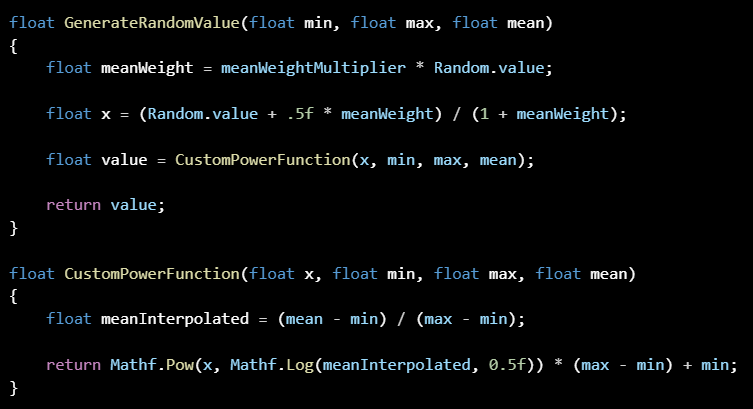
\includegraphics[width=1\textwidth]{images/custom power function c sharp.png}
    \caption{Funkcja CustomPowerFunction, oraz dodatkowa funkcja, która przybliża x do 0.5 na podstawie dodatkowego parametru wagi mediany.}
\end{figure}
Metoda ta pozwala na generowanie wartości losowej dla podanej wartości minimalnej i maksymalnej, a także wybranej mediany. Oznacza to więc, że połowa danych będzie poniżej mediany, a druga połowa powyżej. 
\begin{figure}[H]
    \centering
    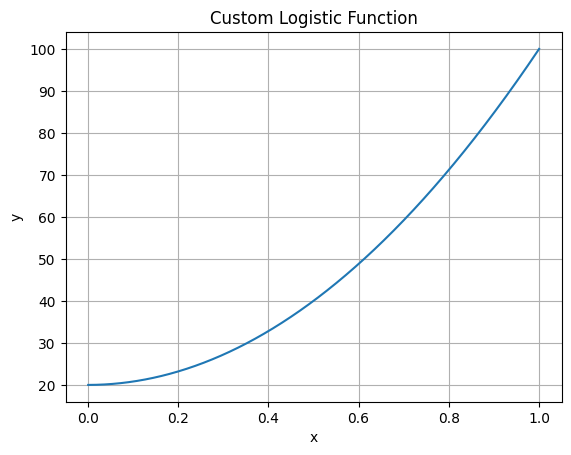
\includegraphics[width=1\textwidth]{images/custom power function graph.png}
    \caption{Rozkład losowanych wartości dla minimum = 20, mediana = 40, maksimum = 100. Podane przykładowe dane są faktycznie używane w grze do ustalenia wielkości mapy.}
\end{figure}

Na początku każdej symulacji tworzony jest plik "Initial settings x - \textit{data i godzina}.csv". Zawarty jest w nim szereg informacji - są to wszystkie parametry, na podstawie których stworzona jest mapa, ustawienia oraz początkowe komórki.
\begin{figure}[H]
    \centering
    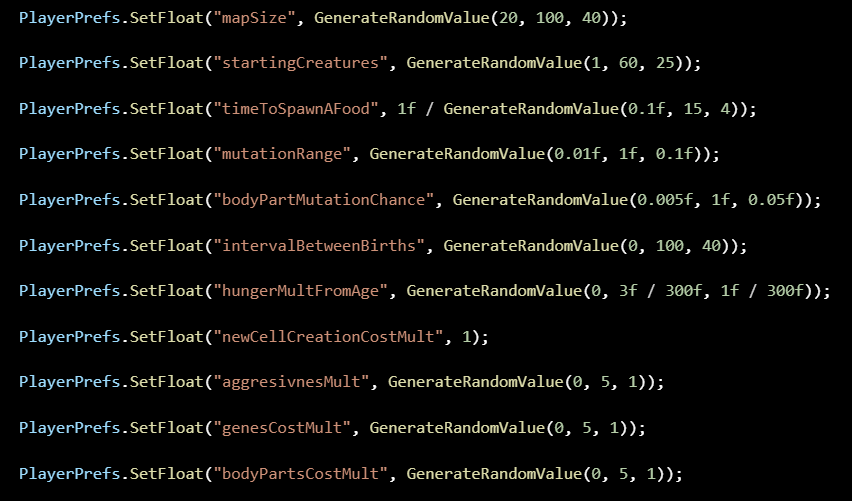
\includegraphics[width=1\linewidth]{images/initial settings injection.png}
    \caption{Parametry ustawiane przy nowych symulacjach, wraz z wartościami minimalnymi, maksymalnymi i domyślnymi.}    
\end{figure}

Następnie zapisywane są dane pozyskane po uruchomieniu symulacji w plikach "Attempt x - \textit{data i godzina}.csv. Co 500 symulowanych sekund zapisane są dane dotyczące ilości komórek, a także wiele średnich - kosztu komórki, genów, a także ilości i rodzaju części ciała. W tym raporcie nie podjęto się analizy zmiany tych wartości w czasie, a jedynie przeanalizowano ostatni wiersz - zapisany zaraz przed końcem symulacji. Taka analiza na pewno również mogłaby być interesująca.

Analizowanym zbiorem danych są więc krotki zawierające dla danej symulacji parametry początkowe oraz ostatni wiersz udokumentowanych rezulatów. Krotki te są formowane w pliku analyzer.py, łączącym pliki "Initial settings x..." i "Attempt x..." na podstawie numeru \textit{x} w nazwie. Ich odczytem zajmuje się biblioteka \href{https://docs.python.org/3/library/csv.html}{\textit{csv}}.

Jedną z pierwszych decyzji było odrzucenie wszystkich symulacji, które zakończyły się przedwcześnie - z powodu wymarcia wszystkich komórek lub nadmiernego wzrostu populacji (ponad 200 komórek żyjących naraz). Decyzja ta była zmotywowana faktem, że dane te zbyt mocno różniłyby się od oczekiwanych i kończyłyby się wcześniej, niż cała reszta.

\begin{figure}[H]
    \centering
    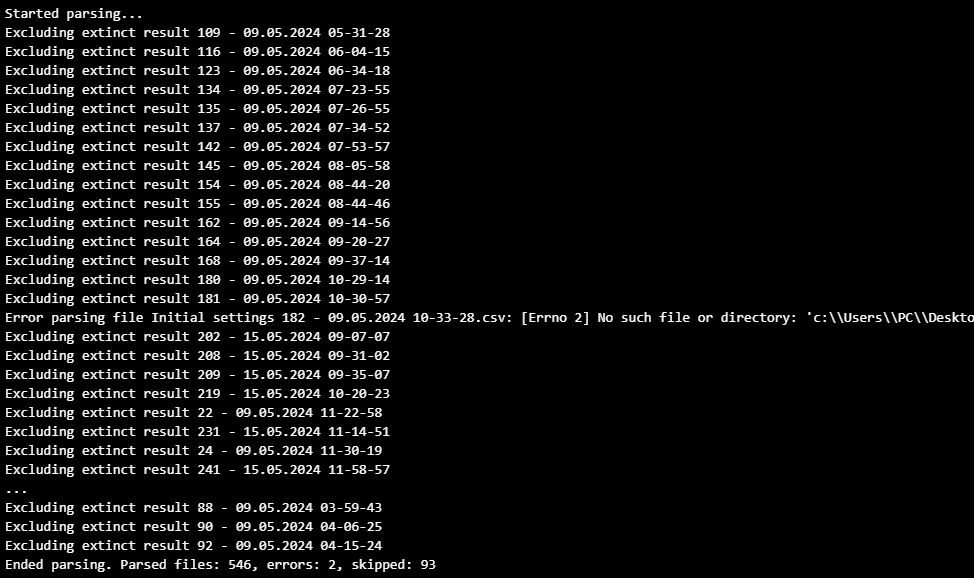
\includegraphics[width=1\linewidth]{images/parse csvs.png}
    \caption{Z 641 wierszy 2 nie miały odpowiadającego im pliku "Attempt x...", a 93 pominięto z powodu przedwczesnego zakończenia. Wśród pominiętych danych, tylko 1 symulacja doświadczyła nadmiernego wzrostu populacji.}    
\end{figure}

\begin{table}[H]
    \begin{tabular}{lllll}
        \toprule
        \textbf{Parametr początkowy} & \textbf{Wartość} \\
        \midrule
        mapSize                             & 23.761980 \\
        startingCreatures                   & 15.000000 \\
        timeToSpawnAFood                    & 4.529128  \\
        hungerMult                          & 0.750000  \\
        speedMult                           & 2.000000  \\
        mitosisSpeedMult                    & 1.000000  \\
        mutationRange                       & 0.383709  \\
        bodyPartMutationChance              & 0.005873  \\
        intervalBetweenBirths               & 64.644820 \\
        hungerMultFromAge                   & 0.003437  \\
        newCellCreationCostMult             & 1.000000  \\
        aggresivnesMult                     & 1.202730  \\
        genesCostMult                       & 0.254597  \\
        bodyPartsCostMult                   & 0.791882  \\
        initialSize                         & 0.300000  \\
        fullyRandomiseStartingGenes         & 0  \\
        allCreaturesStartAsDesignedCreature & 0  \\
        startAsACreature                    & 0  \\
        colorfulCells                       & 0  \\
        speedGeneOn                         & 1  \\
        sensorGeneOn                        & 1  \\
        processingGeneOn                    & 1  \\
        gluttonyGeneOn                      & 1  \\
        reproductionGeneOn                  & 1  \\
        storageGeneOn                       & 1  \\
        parentEmpathyGeneOn                 & 1  \\
        aggresivnessGeneOn                  & 1  \\
        healthGeneOn                        & 1  \\
        foodPreferenceGeneOn                & 0  \\
        fightingPermitted                   & 1  \\
         \bottomrule
    \end{tabular}
    \caption{Przykładowe wartości parametrów początkowych.}
\end{table}

\begin{table}[H]
    \begin{tabular}{lllll}
        \toprule
        \textbf{Rezultat} & \textbf{Wartość} \\
        \midrule
        simulation time                     & 4500.051000 \\
        speed gene                          & 0.991227    \\
        sensor gene                         & 0.416732    \\
        processing gene                     & 0.814775    \\
        gluttony gene                       & 0.573346    \\
        reproduction wilness gene           & 0.307748    \\
        energy storage capacity gene        & 0.733310    \\
        parental empathy gene               & 0.345123    \\
        aggresivness gene                   & 0.866806    \\
        health gene                         & 0.861556    \\
        food preference gene                & 0.500000    \\
        creatures count                     & 18   \\
        average creature cost               & 41.878194   \\
        average amount of body parts        & 0.000000    \\
        average amount of protective spikes & 0.000000    \\
        average amount of composters        & 0.000000    \\
        average amount of turbines          & 0.000000    \\
        average amount of offensive spikes  & 0.000000    \\
    \end{tabular}
    \caption{Przykładowe wartości rezultatów.}
\end{table}

\subsection{Oczyszczanie danych}
Przed właściwą analizą danych, wymagają one wstępnego przetworzenia i oczyszczenia.

Wiele kolumn będzie można usunąć z powodu braku ich istotności. Najpierw warto przeanalizować macierze korelacji obu tabel.

\begin{figure}[H]
    \centering
    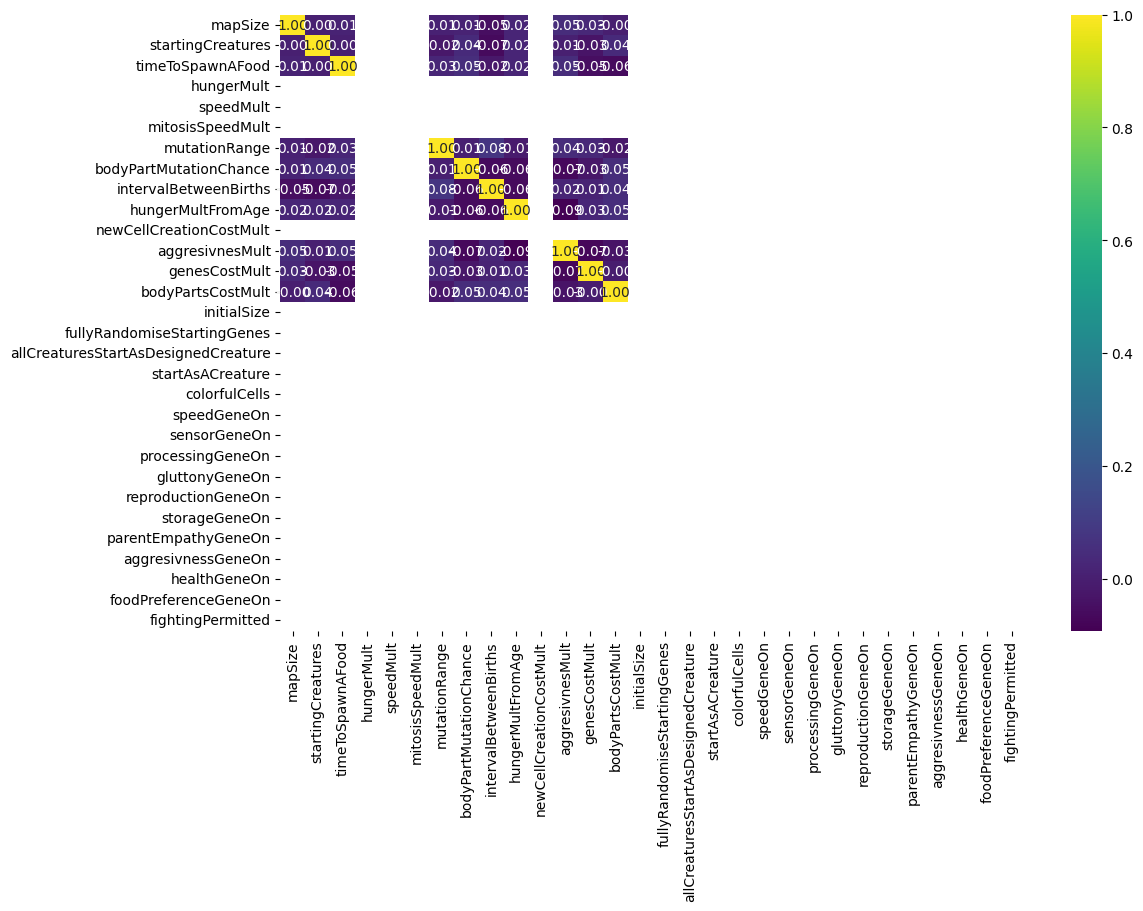
\includegraphics[width=0.85\linewidth]{images/initials correlation raw.png}
    \caption{Macierz korelacji parametrów początkowych przed ich oczyszczeniem.}
\end{figure}

\begin{figure}[H]
    \centering
    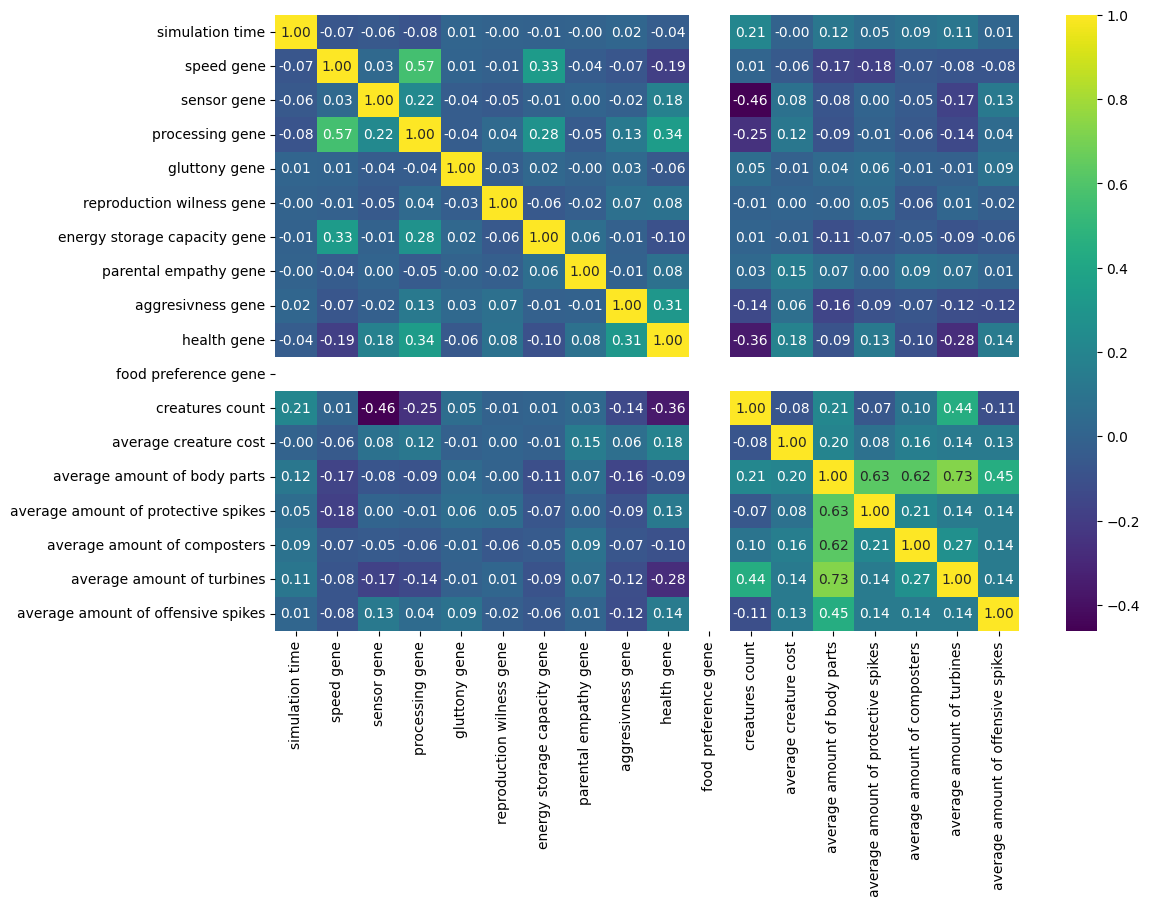
\includegraphics[width=0.85\linewidth]{images/results correlation raw.png}
    \caption{Macierz korelacji rezultatów przed ich oczyszczeniem.}
\end{figure}

Oczywistym wnioskiem jest usunięcie danych, które są stałe dla każdej symulacji. Są to białe wiersze/kolumny. Dodatkowo usunięta została kolumna "simulation time", ponieważ jej wartości zawsze będą zbliżone do 4500.

\section{Analiza i dalsze przetwarzanie przygotowanych danych}

\subsection{Eksploracyjna analiza danych}
\begin{figure}[H]
    \centering
    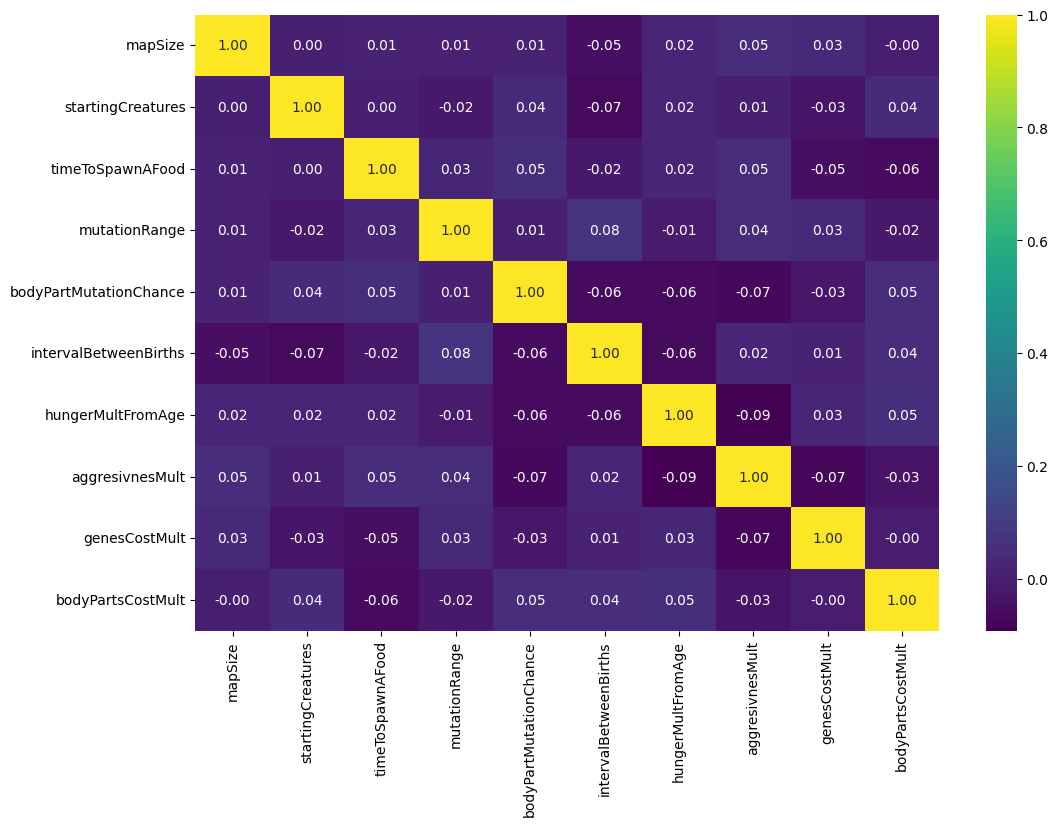
\includegraphics[width=0.5\linewidth]{images/initials correlation cleaned.png}
    \caption{Macierz korelacji parametrów początkowych.}
\end{figure}

Ponieważ dane były generowane losowo w sposób niezależny od siebie, korelacje parametrów początkowych w zależności od innych są bliskie 0. Był to oczekiwany rezultat.

\begin{figure}[H]
    \centering
    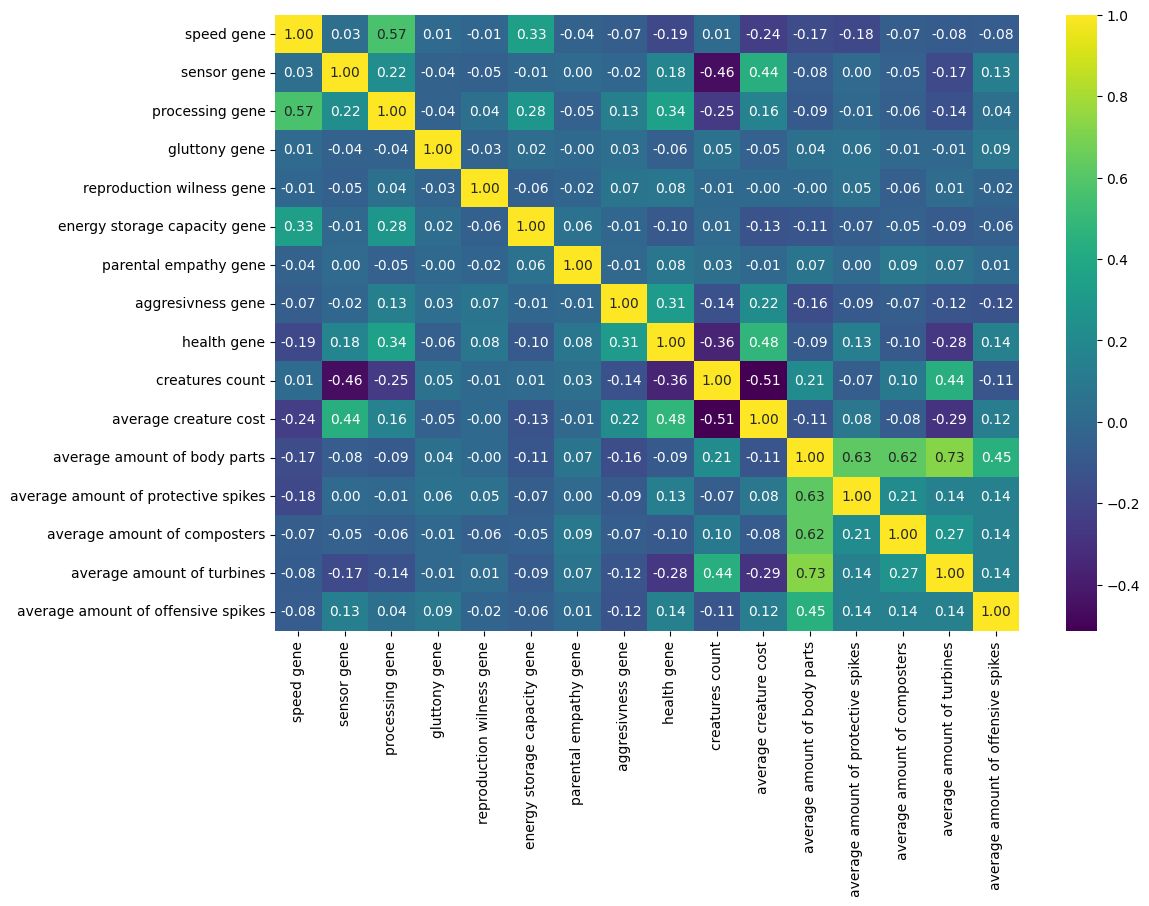
\includegraphics[width=1\linewidth]{images/results correlation cleaned.png}
    \caption{Macierz korelacji rezultatów.}
\end{figure}

W tej macierzy korelacji można zaobserwować wiele interesujących zależności. Oto niektóre z nich:

Niektóre z nich są oczywiste – średnia liczba części ciała jest oparta na średnich ilościach innych części ciała. Istnienie części ciała może oznaczać, że parametr początkowy odpowiadający za szansę mutacji części ciała jest wyższy, co sprawia, że istnienie innych części staje się bardziej prawdopodobne.

Występuje silna korelacja między genem przetwarzania jedzenia, a genem prędkości. Przy większej liczbie stworzeń, mniej korzystne jest posiadanie lepiej rozwiniętego genu sensorycznego.

Interesującą, silną korelacją jest ta między liczbą stworzeń a średnią liczbą turbin. Wydaje się, że przy większej liczbie stworzeń ważne jest, aby dotrzeć do jedzenia przed innymi. Z drugiej strony, ta sama korelacja nie jest obserwowana między liczbą stworzeń a genem prędkości. Jednym z powodów może być niezamierzony błąd w grze – dane były zbierane przy prędkości symulacji wynoszącej 16, co jest dość dużą wartością. Z tego powodu stworzenia o dużej prędkości mogą „mijać” jedzenie, ponieważ mają mniej klatek do dostosowania swojego kierunku ruchu. Turbiny znacznie zwiększają prędkość skręcania, podczas gdy gen prędkości tego nie robi. Możliwe więc jest to, że wartości te byłyby inne dla mniejszej prędkości symulacji. Innym wytłumaczeniem mogłoby być to, że turbiny energetycznie opłacają się bardziej niż gen szybkości.

Jedyną daną z rezultatów, która pozostanie, jest średni koszt komórek. W następnym dziale przeprowadzona będzie estymacja tej kolumny nie tylko z parametrów początkowych, ale też z reszty rezultatów.

\subsection{Usuwanie wartości odstających (outlierów)}

\begin{figure}[H]
    \centering
    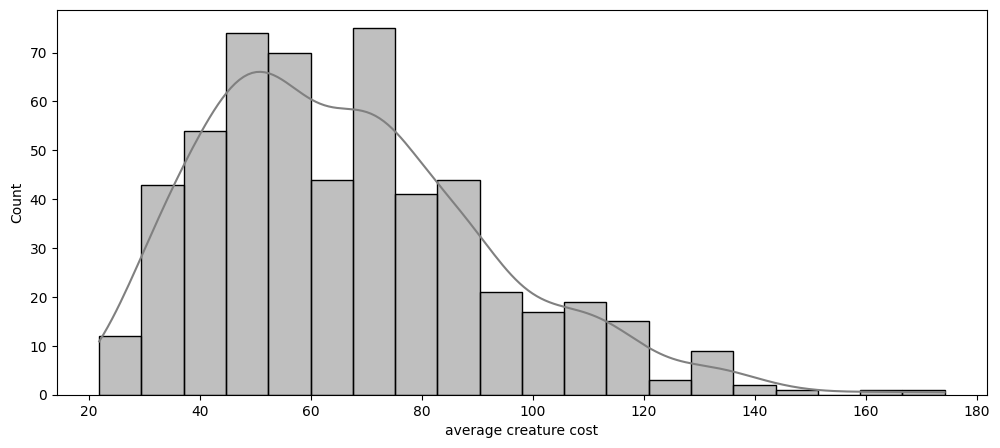
\includegraphics[width=1\linewidth]{images/creature cost graph.png}
    \caption{Histogram średnich kosztów komórek, wraz z wartościami odstającymi.}    
\end{figure}

Przy pomocy reguły trzech sigm wiersze, dla których średni koszt komórek odstawał w sposób zbyt znaczący od normy, zostały usunięte. W praktyce oznacza to, że około 0.3\% najbardziej odstających danych zostało usunięte, czyli te, których średni koszt komórek był większy od około 140.

\begin{figure}[H]
    \centering
    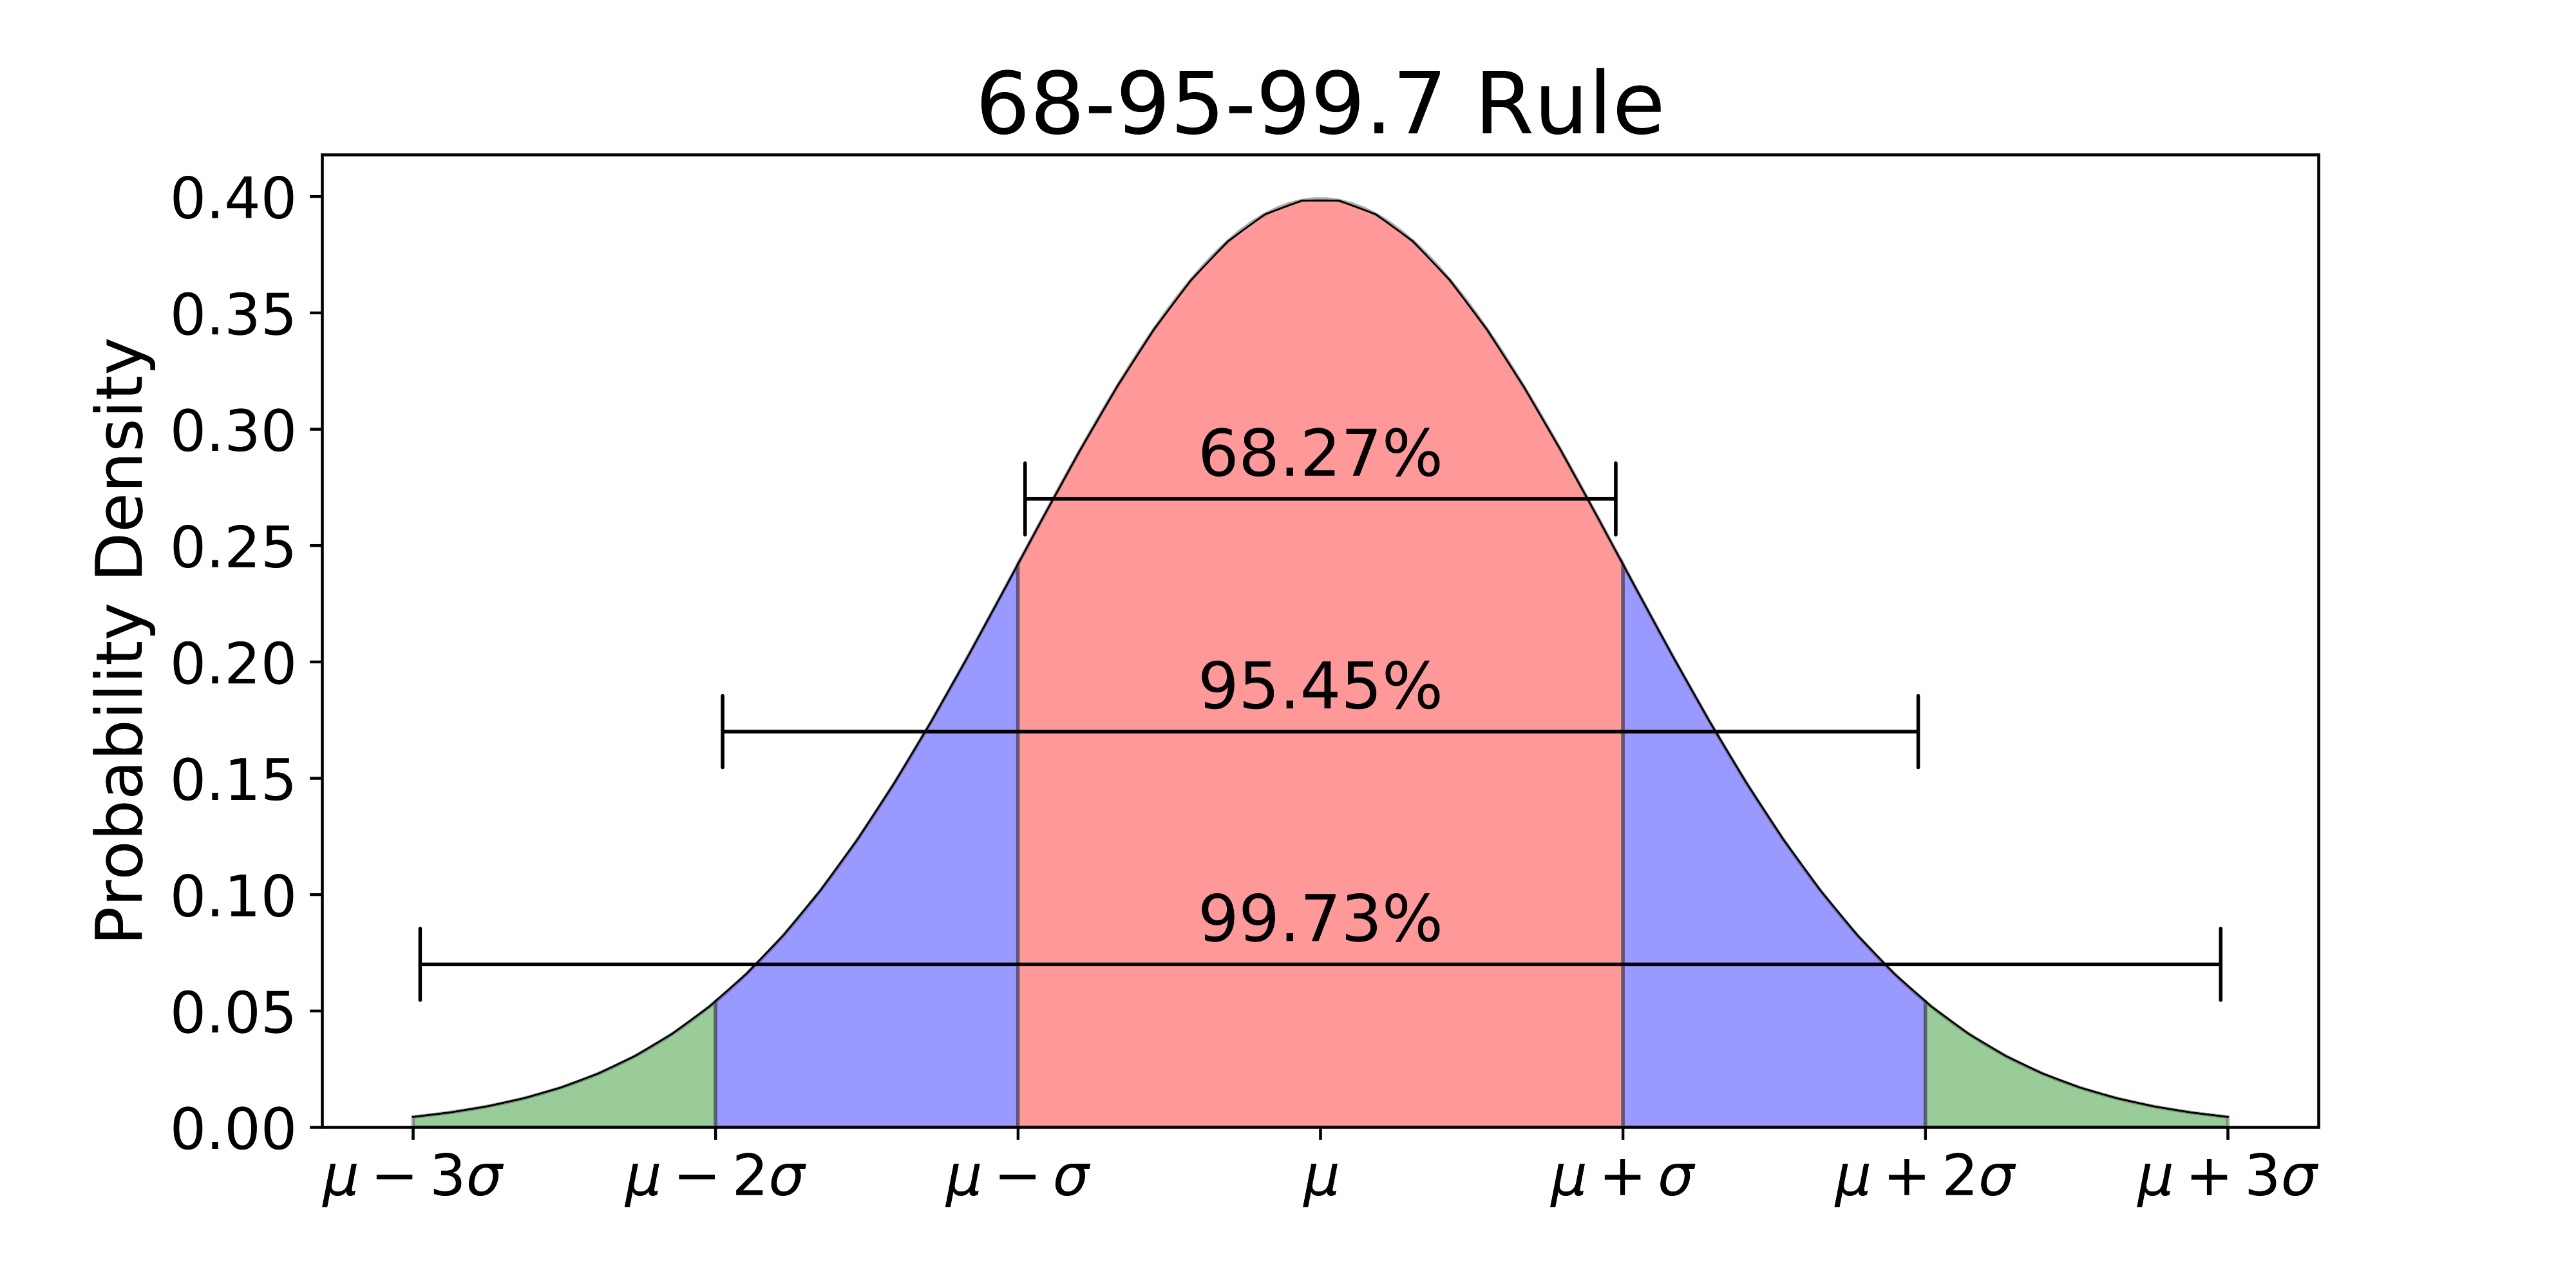
\includegraphics[width=0.75\linewidth]{images/three sigma rule.png}
    \caption{Reguła trzech sigm}
    \label{plt:three_sigm_rule}
\end{figure}

\begin{figure}[H]
    \centering
    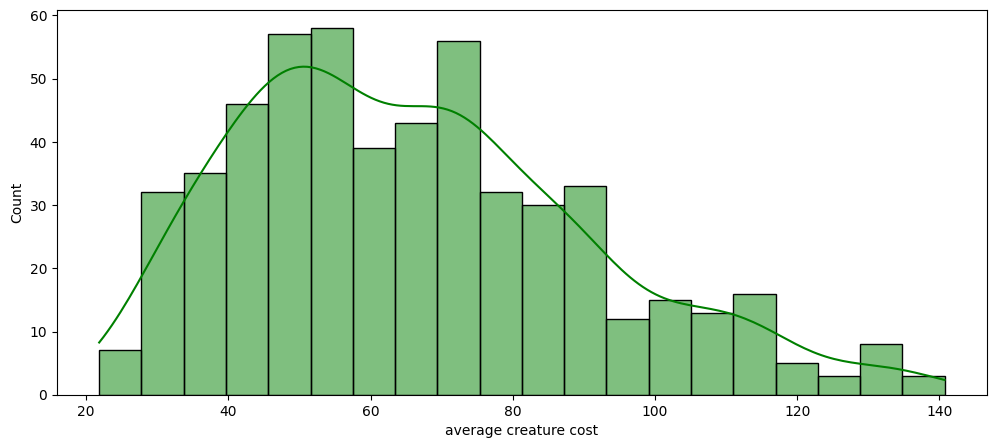
\includegraphics[width=1\linewidth]{images/histogram of average creature cost without outliers.png}
    \caption{Histogram średnich kosztów komórek, bez wartości odstających.}    
\end{figure}

\subsection{Ogólna jakość danych}
Ponieważ dane zostały wytworzone w sposób kontrolowany, nie ma wśród nich nieprawidłowości często spotykanych przy analizie danych pobranych z internetu. Nie występują zduplikowane ani fałszywe wartości. Jedynym problemem był dodatkowy znak ";" w nagłówkach plików .csv. Został on usunięty ze wszystkich plików.

\subsection{Estymacja rezultatów z parametrów początkowych}
Za pomocą modelu \href{https://scikit-learn.org/stable/modules/generated/sklearn.linear_model.LinearRegression.html}{LinearRegression z modułu sklearn} przeprowadzono estymację różnych rezultatów z parametrów początkowych. Podane wyniki to wskaźnik \( R^2 \).
\begin{table}[H]
    \centering
    \begin{tabular}{lr}
        \toprule
        \textbf{Gene/Metric} & \textbf{Estimation score} \\
        \midrule
        Speed gene & 0.2966 \\
        Sensor gene & 0.2700 \\
        Processing gene & 0.5678 \\
        Gluttony gene & 0.0168 \\
        Reproduction wilness gene & -0.0006 \\
        Energy storage capacity gene & 0.1768 \\
        Parental empathy gene & 0.0567 \\
        Aggressiveness gene & 0.0751 \\
        Health gene & 0.4507 \\
        Creatures count & 0.6871 \\
        Average creature cost & 0.8060 \\
        Average amount of body parts & 0.4945 \\
        Average amount of protective spikes & 0.2272 \\
        Average amount of composters & 0.2165 \\
        Average amount of turbines & 0.3628 \\
        Average amount of offensive spikes & 0.1533 \\        
        \bottomrule
    \end{tabular}
    \caption{Tabela wyniku estymacji rezultatów z parametrów początkowych.}
\end{table}
Z tych danych wyciągnięto następujące wnioski:
\begin{enumerate}
    \item Najwyższy wynik regresji był dla średniego kosztu komórek - 0,8060.
    \item Wyniki regresji niektórych innych rezultatów osiągnęły umiarkowanie wysokie wartości - w tym dla genu przetwarzania jedzenia, genu zdrowia czy też średniej ilości części ciała, 
    \item Większość regresji osiągnęła wynik niski lub bardzo niski.
\end{enumerate}
Dane analizowane w raporcie dotyczą średniego kosztu komórki, który osiągnął wynik około 0,8. Wynik ten sugeruje, że zależność między tą daną a parametrami początkowymi jest dość silna.

\section{Regresja liniowa na podstawie parametrów początkowych}

\subsection{Kolumna korelacji}
\begin{figure}[H]
    \centering
    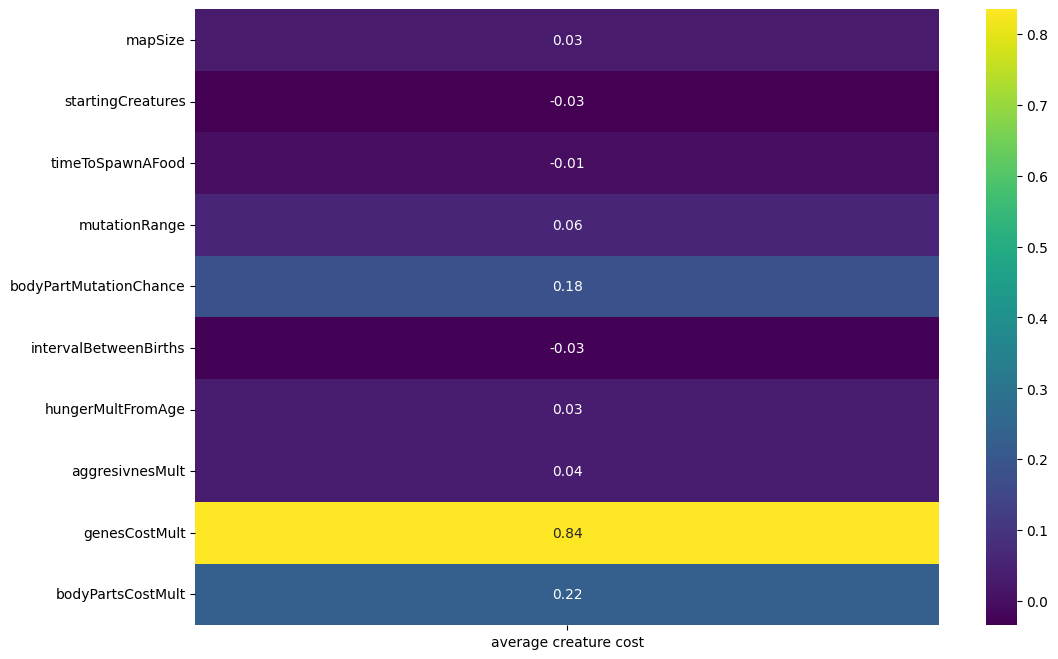
\includegraphics[width=1\linewidth]{images/correlation column average cost from initials.png}
    \caption{Kolumna korelacji średniego kosztu komórki od parametrów początkowych symulacji.}    
\end{figure}

Ponieważ wartość korelacji jest niska dla wielu kolumn, estymacja powstanie na bazie tylko trzech parametrów początkowych. Wybrane zostały:
\begin{itemize}
    \item mnożnik agresywności
    \item czas między powstaniem jedzenia
    \item mnożnik kosztu genów
\end{itemize}
\label{correlation-items1}

\subsection{Wynik regresji liniowej}
\label{regression-from-initial-parameters}
Po przeskalowawaniu danych za pomocą \href{https://scikit-learn.org/stable/modules/generated/sklearn.preprocessing.StandardScaler.html}{StandardScaler}, oto wyniki regresji:
\begin{table}[H]
    \centering
    \begin{tabular}{lr}
        \toprule
        \textbf{Data type} & \textbf{\(R^2\)} \\
        \midrule        
        Test data & 0.7631864002167397 \\
        Train data & 0.7937762753894901 \\ 
        \bottomrule
    \end{tabular}
    \label{tab:genetic_metrics}
\end{table}

\subsection{Wykresy wartości parametrów początkowych, a średniego kosztu komórki}

\begin{figure}[H]
    \centering
    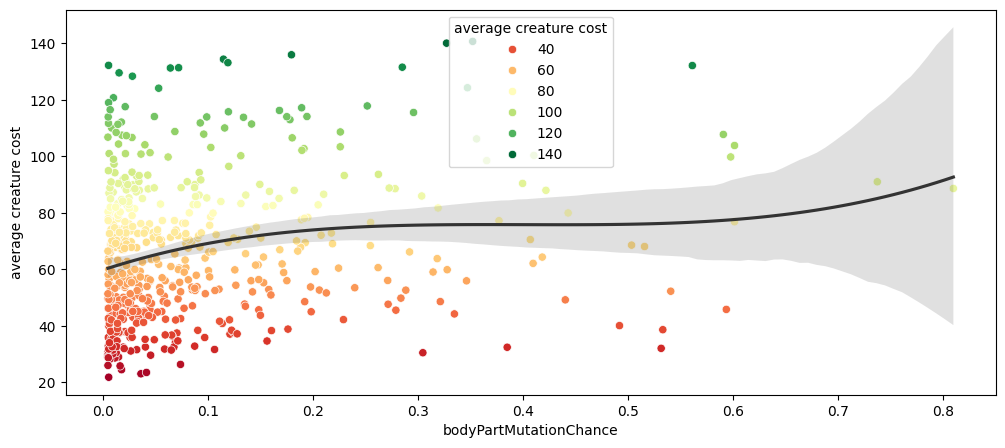
\includegraphics[width=1\linewidth]{images/body part mutation chance graph.png}
    \caption{Wykres szansy mutacji części ciała, a średniego kosztu komórki.}
    \label{fig:mutation-chance1}
\end{figure}

Jak widać na wykresie, występuje pewna korelacja. Nie jest ona silna. Niepewność również wzrasta, do bardzo wysokiego poziomu.

\begin{figure}[H]
    \centering
    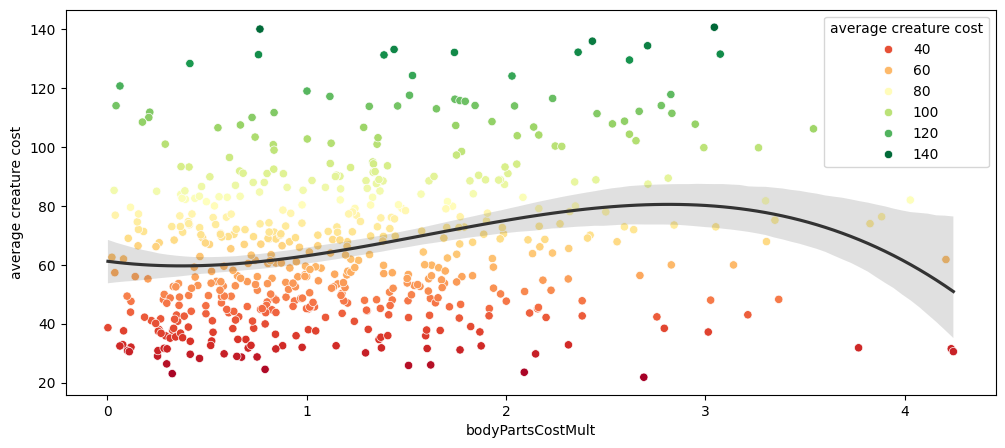
\includegraphics[width=1\linewidth]{images/body parts cost mult graph.png}
    \caption{Wykres mnożnika kosztu części ciała, a średniego kosztu komórki.}
    \label{fig:body-cost-mult1}
\end{figure}

Jak widać na wykresie, średni koszt komórki wzrasta razem z mnożnikiem kosztu części ciała, aż do czasu. Potem zaczyna się obniżać. Być może to przez to, że gdy koszt części ciała jest tak wysoki, komórki wymierają, co może sprawiać, że przeżyją tylko te, które mogą reprodukować się najniższym kosztem.

\begin{figure}[H]
    \centering
    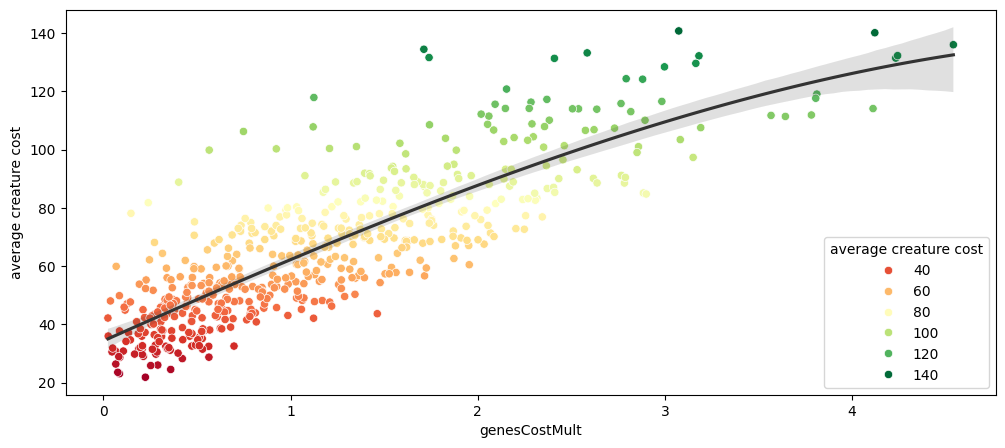
\includegraphics[width=1\linewidth]{images/genes cost mult graph.png}
    \caption{Wykres mnożnika kosztu genów, a średniego kosztu komórki.}
    \label{fig:gene-cost-mult1}
\end{figure}

Korelacja jest bardzo silna i liniowa. Dopiero przy najwyższych wartościach mnoznika kosztu genów koszt komórek zaczyna wolniej rosnąć, co może być spowodowane ewolucją i przetrwaniem tylko tych, którzy mogą wydać potomstwo z mniejszą inwestycją energetyczną.

\subsection{Wnioski z estymacji średniego kosztu komórki z początkowych parametrów}

Okazuje się, że występuje bardzo silna korelacja między średnim kosztem komórki, a mnoznikiem kosztu genów. Widoczna jest również korelacja między szansą mutacji części ciała czy mnoznikiem kosztu części ciała. Wynik regresji na poziomie 0,8 jest wysoki, biorąc pod uwagę ilość losowości w symulacji. Nie wygląda na to, aby doszło do nadmiernego dopasowania (overfittingu) - wyniki estymatorów dla danych treningowych są równie wysokie.

\section{Regresja liniowa na podstawie rezultatów i parametrów początkowych}

Skoro mamy dane pozostałych rezultatów, interesujące byłoby sprawdzić, jak dołączenie tych danych wpłynęłoby na estymację kosztu komórek.

\subsection{Kolumna korelacji}
\begin{figure}[H]
    \centering
    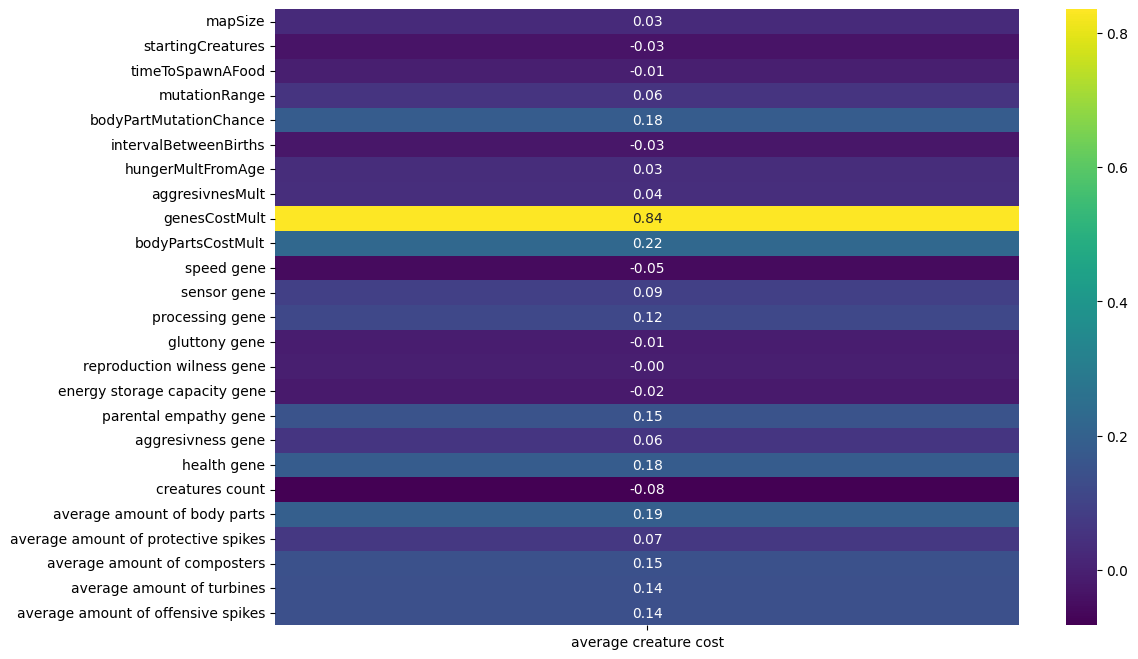
\includegraphics[width=1\linewidth]{images/correlation column average creature cost all parameters.png}
    \caption{Kolumna korelacji średniego kosztu komórki od parametrów początkowych symulacji i rezultatów.}    
\end{figure}

Ponieważ wartość korelacji jest niska dla wielu kolumn, estymacja powstanie na bazie tylko niektórych parametrów początkowych i rezultatów. Do poprzednich parametrów (\ref{correlation-items1}) dodane zostały:
\begin{itemize}
    \item średnia wartość genu szybkości
    \item średnia wartość genu sensorycznego
    \item średnia wartość genu przetwarzania jedzenia
    \item średnia wartość genu łakomstwa
    \item średnia wartość genu empatii rodzicielskiej
    \item średnia wartość genu agresji
    \item średnia wartość genu zdrowia
    \item średnia ilość części ciała
    \item średnia ilość kolców ochronnych
    \item średnia ilość kompostowników
    \item średnia ilość turbin
    \item średnia ilość kolców ofensywnych
\end{itemize}

\subsection{Wynik regresji liniowej}

Skalując dane za pomocą \href{https://scikit-learn.org/stable/modules/generated/sklearn.preprocessing.StandardScaler.html}{StandardScaler}, oto wyniki regresji:
\begin{table}[H]
    \centering
    \begin{tabular}{lr}
        \toprule
        \textbf{Regression Score on: } & \textbf{\(R^2\)} \\
        \midrule        
        Test data & 0.9023 \\
        Train data & 0.9124 \\
        Full data & 0.9103 \\    
        \bottomrule
    \end{tabular}
\end{table}

\subsection{Wykresy wartości parametrów początkowych i rezultatów, a średniego kosztu komórki}

3 wykresy pojawiły się już w poprzednim dziale:
\ref{fig:body-cost-mult1}
\ref{fig:gene-cost-mult1}
\ref{fig:mutation-chance1}

\begin{figure}[H]
    \centering
    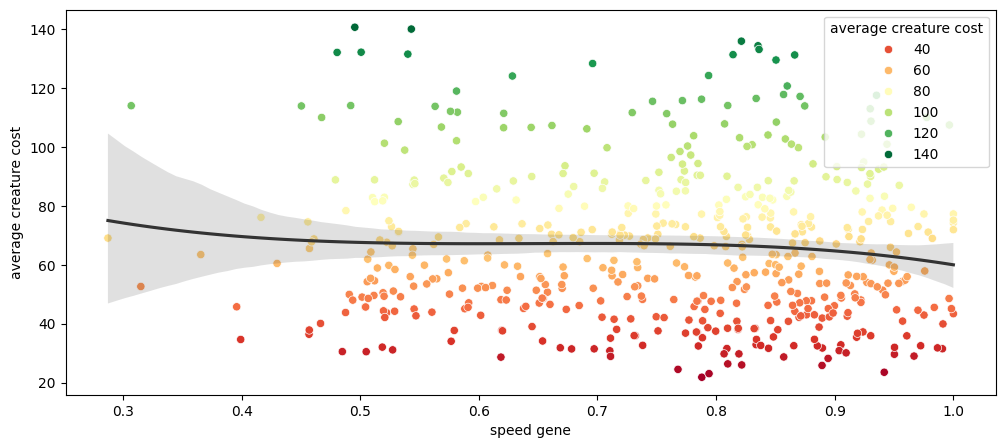
\includegraphics[width=0.8\linewidth]{images/speed gene graph results.png}
    \caption{Wykres średniej wartości genu szybkości, a średniego kosztu komórki.}
\end{figure}

\begin{figure}[H]
    \centering
    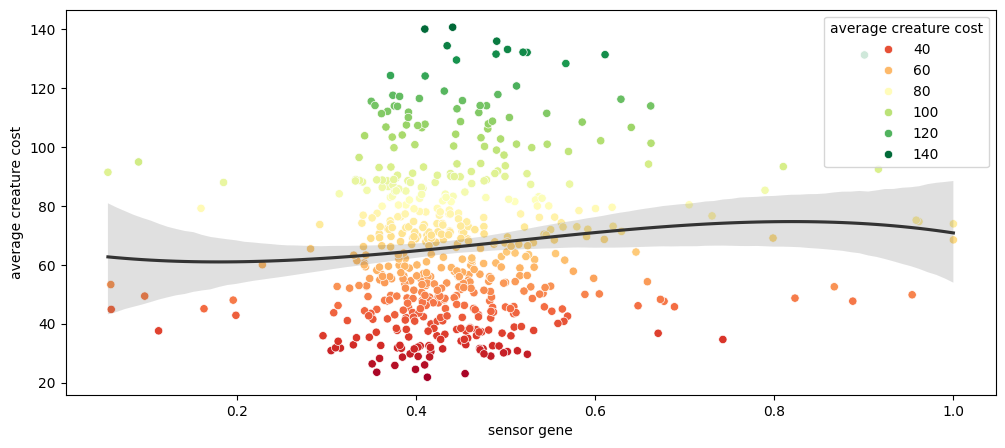
\includegraphics[width=0.8\linewidth]{images/sensor gene graph results.png}
    \caption{Wykres średniej wartości genu sensorycznego, a średniego kosztu komórki.}
\end{figure}

\begin{figure}[H]
    \centering
    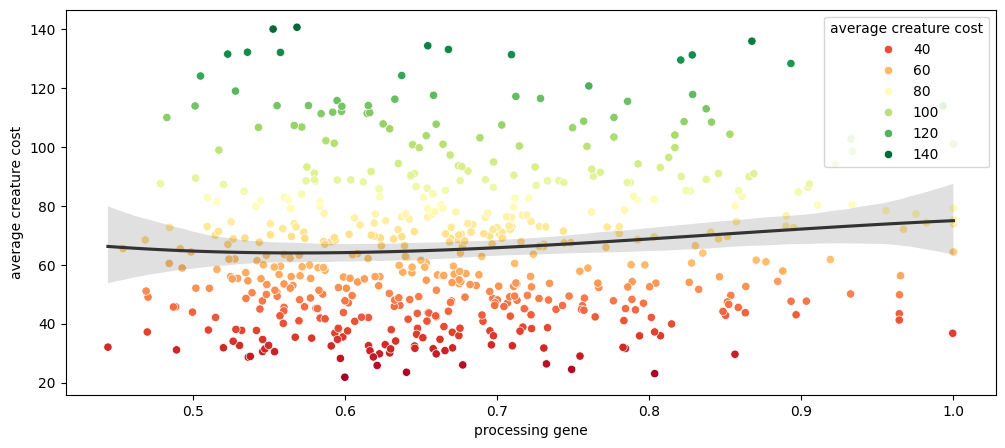
\includegraphics[width=0.8\linewidth]{images/processing gene graph results.png}
    \caption{Wykres średniej wartości genu przetwarzania jedzenia, a średniego kosztu komórki.}
\end{figure}

\begin{figure}[H]
    \centering
    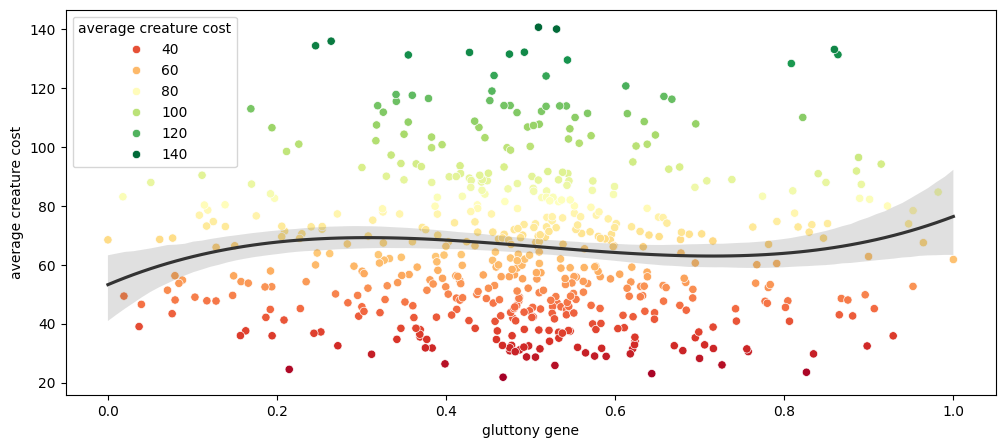
\includegraphics[width=0.8\linewidth]{images/gluttony gene graph results.png}
    \caption{Wykres średniej wartości genu łakomstwa, a średniego kosztu komórki.}
\end{figure}

\begin{figure}[H]
    \centering
    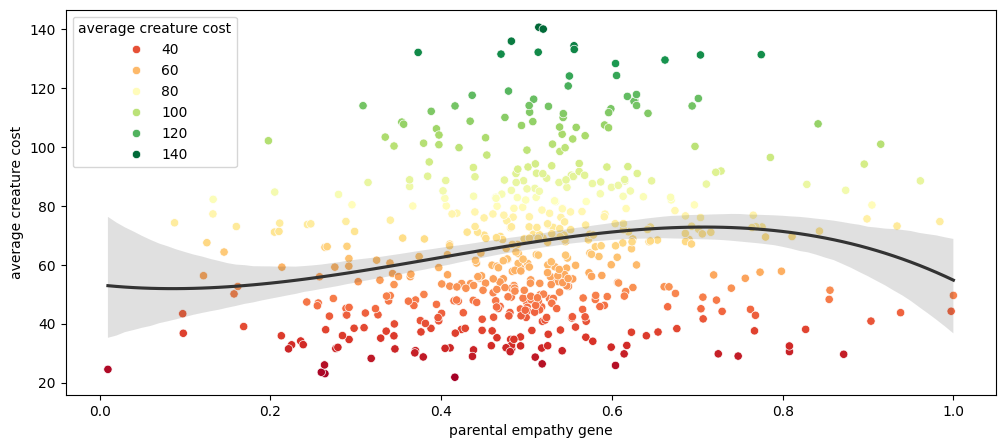
\includegraphics[width=0.8\linewidth]{images/parental empathy gene graph results.png}
    \caption{Wykres średniej wartości genu empatii rodzicielskiej, a średniego kosztu komórki.}
\end{figure}

\begin{figure}[H]
    \centering
    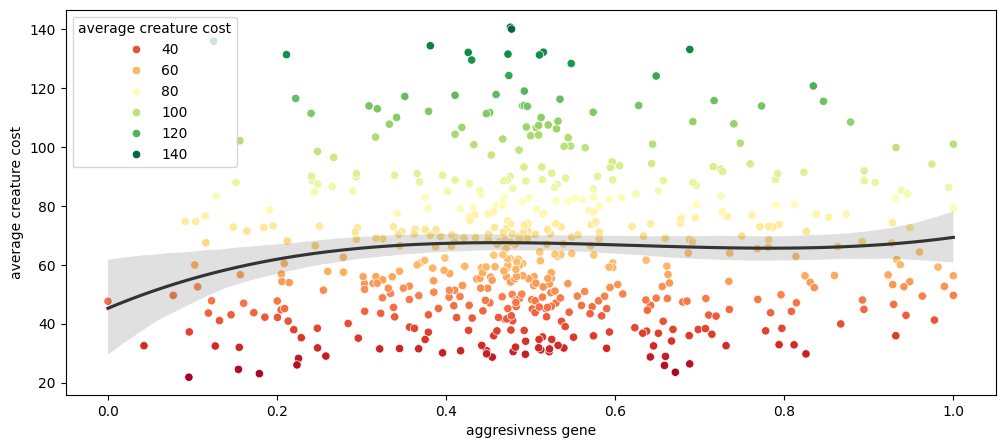
\includegraphics[width=0.8\linewidth]{images/aggresivness gene graph results.png}
    \caption{Wykres średniej wartości genu agresji, a średniego kosztu komórki.}
\end{figure}

\begin{figure}[H]
    \centering
    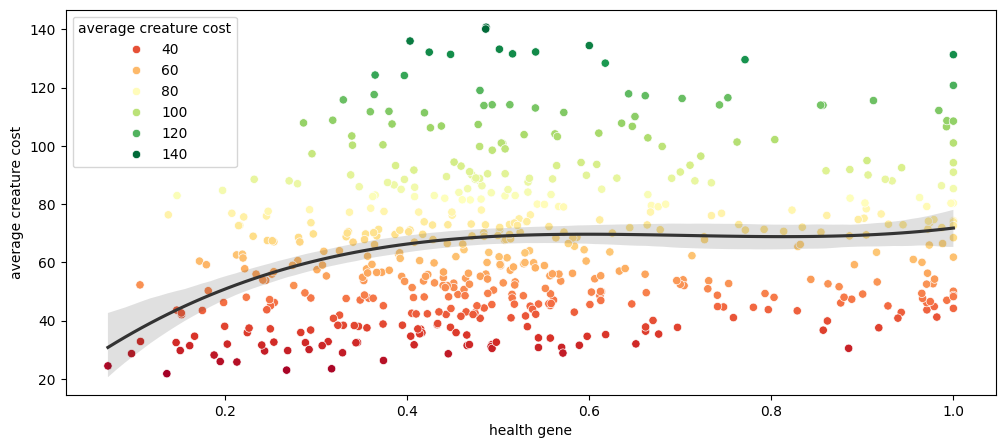
\includegraphics[width=0.8\linewidth]{images/health gene graph results.png}
    \caption{Wykres genu zdrowia, a średniego kosztu komórki.}
\end{figure}

\begin{figure}[H]
    \centering
    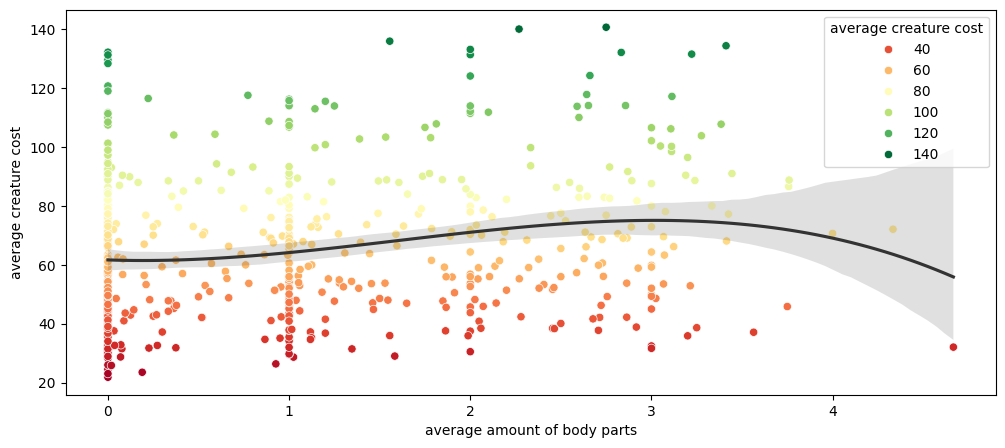
\includegraphics[width=0.8\linewidth]{images/average amount of body parts graph results.png}
    \caption{Wykres średniej ilości części ciała, a średniego kosztu komórki.}
\end{figure}

\begin{figure}[H]
    \centering
    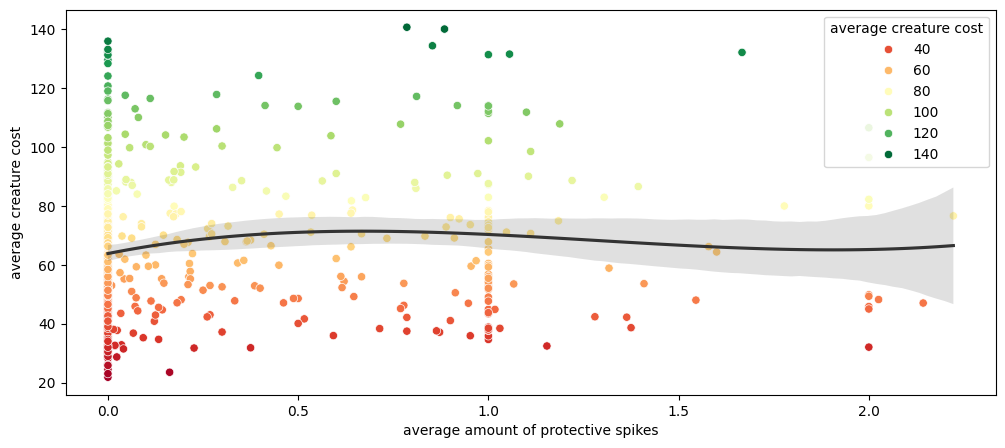
\includegraphics[width=0.8\linewidth]{images/average amount of protective spikes graph results.png}
    \caption{Wykres średniej ilości kolców ochronnych, a średniego kosztu komórki.}
\end{figure}

\begin{figure}[H]
    \centering
    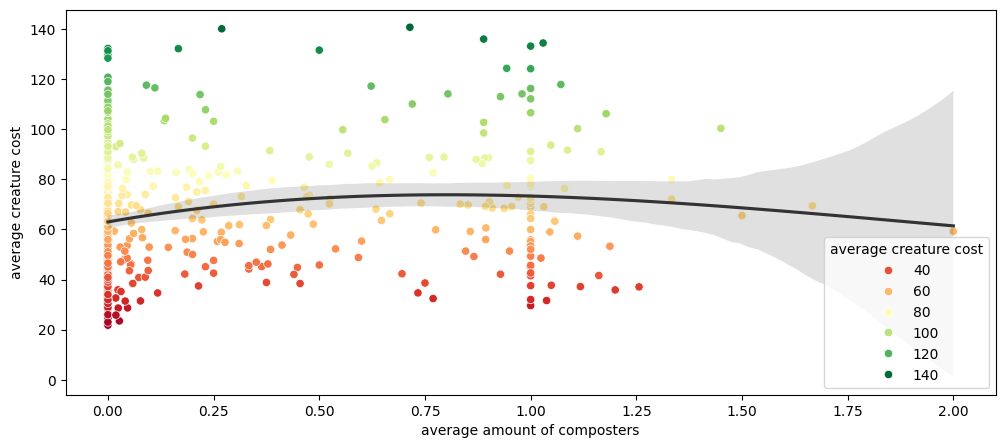
\includegraphics[width=0.8\linewidth]{images/average amount of composters graph results.png}
    \caption{Wykres średniej ilości kompostowników, a średniego kosztu komórki.}
\end{figure}

\begin{figure}[H]
    \centering
    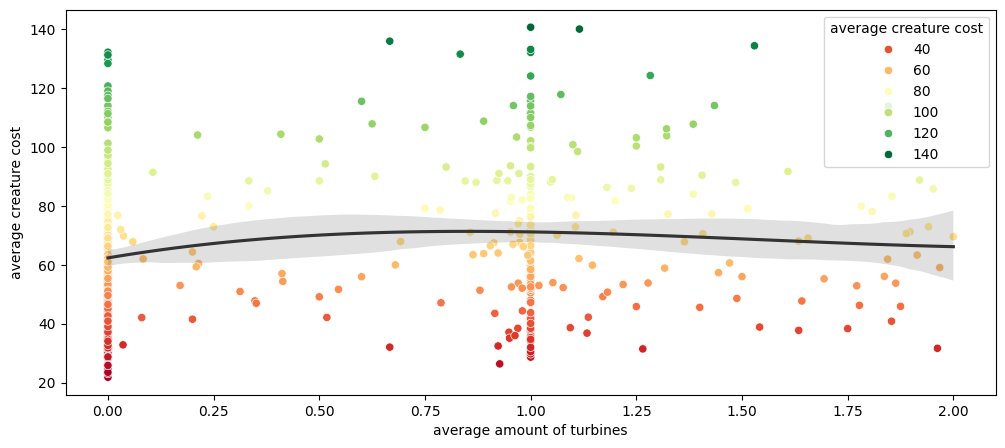
\includegraphics[width=0.8\linewidth]{images/average amount of turbines graph results.png}
    \caption{Wykres średniej ilości turbin, a średniego kosztu komórki.}
\end{figure}

\begin{figure}[H]
    \centering
    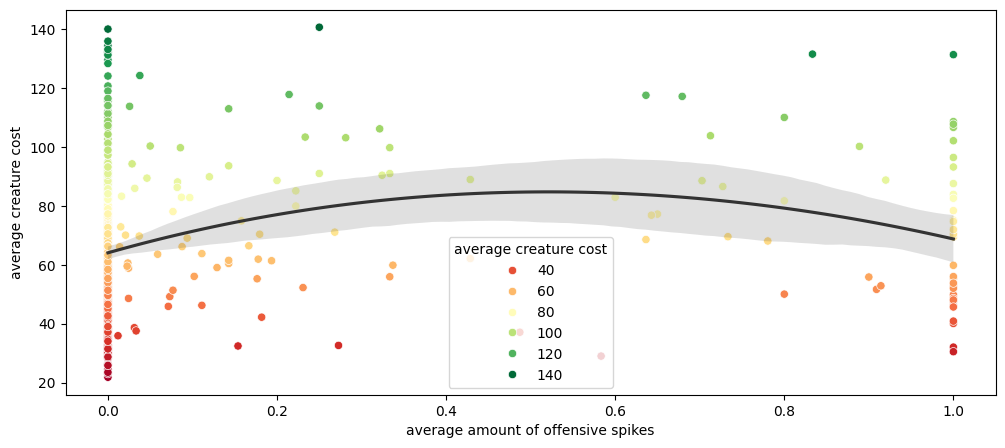
\includegraphics[width=0.8\linewidth]{images/average amount of offensive spikes graph results.png}
    \caption{Wykres średniej ilości kolców ofensywnych, a średniego kosztu komórki.}
\end{figure}

Patrząc na wykresy średnich ilości ciała, widać anomalie wśród danych - wiele tych średnich wartości to liczby całkowite. Jest to jednak oczekiwane, gdyż pod koniec symulacji może się zdarzyć, że pozostanie niewielka liczba komórek, wszystkie mające tą samą ilość części ciała.

\subsection{Wnioski z estymacji średniego kosztu komórki z rezultatów i początkowych parametrów}

Wysokość korelacji uległa poprawie w porównaniu z estymacją z samych rezultatów, z poziomu 0,8 do około 0,9. Jest to wysoki wynik, biorąc pod uwagę ilość losowości w symulacji. Nadal widać jednak, że to sam mnożnik kosztu genów odpowiada za dużą część tego wyniku. Ilość analizowanych danych również się mocno zwiększyła. Nie wygląda na to, aby doszło do nadmiernego dopasowania (overfittingu) -- wyniki estymatorów dla danych treningowych są równie wysokie. 

\section{Porównanie estymacji wśród różnych modeli}
Ostatnim etapem było ponowna estymacja kosztu komórek na podstawie samych parametrów początkowych, ale z użyciem różnych modeli. Wybrane zostały trzy, które osiągnęły najlepsze wyniki.

\subsection{Testowanie modeli}

\begin{figure}[H]
    \centering
    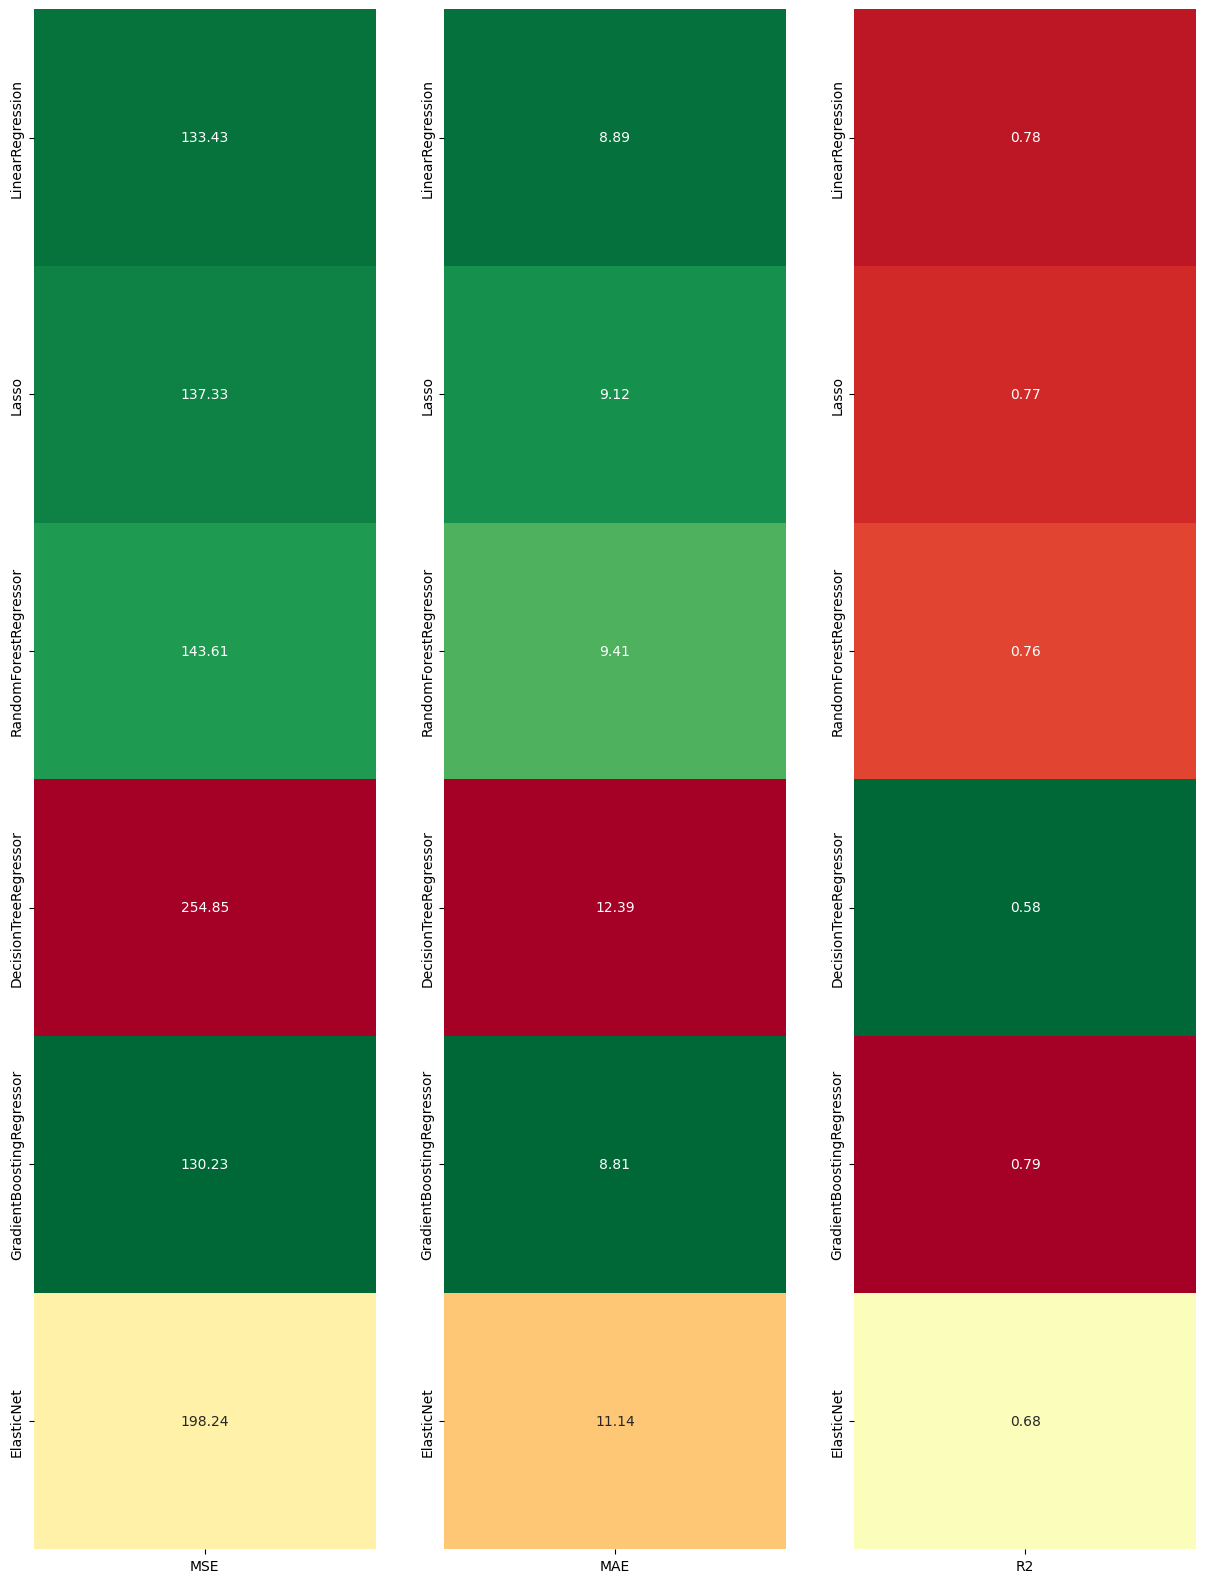
\includegraphics[width=0.8\linewidth]{images/models tested.png}
    \caption{Wartości MSE, MAE i \(R^2\) dla przetestowanych modeli.}
\end{figure}

Na danych z działu \nameref{regression-from-initial-parameters} przetestowano następujące modele:
LinearRegression, \href{https://scikit-learn.org/stable/modules/generated/sklearn.linear_model.Lasso.html}{Lasso}, 
\href{https://scikit-learn.org/stable/modules/generated/sklearn.ensemble.RandomForestRegressor.html}{RandomForestRegressor}, \href{https://scikit-learn.org/stable/modules/generated/sklearn.tree.DecisionTreeRegressor.html}{DecisionTreeRegressor}, \href{https://scikit-learn.org/stable/modules/generated/sklearn.ensemble.GradientBoostingRegressor.html}{GradientBoostingRegressor} i \href{https://scikit-learn.org/stable/modules/generated/sklearn.linear_model.ElasticNet.html}{ElasticNet}. 
Stworzona została heatmapa, zawierająca miary \href{https://help.qlik.com/pl-PL/cloud-services/Subsystems/Hub/Content/Sense_Hub/AutoML/scoring-regression.htm}{MSE, MAE i \(R^2\)} przetestowanych modeli. 
Po przeanalizowaniu wyników, do analizy wybrano LinearRegression, RandomForestRegressor i GradientBoostingRegressor.

\subsection{Szukanie najlepszych parametrów modeli}
Każdy model przyjmuje inne parametry, decydujące o poziomie jego dopasowania do danych. 

\subsubsection{Linear Regression}
Regresja liniowa z cechami wielomianowymi \cite{polynomial_features} to technika uczenia maszynowego, która rozszerza możliwości tradycyjnej regresji liniowej poprzez uwzględnienie wielomianowych przekształceń cech wejściowych. Dzięki temu model może uchwycić nieliniowe zależności między zmiennymi niezależnymi a zmienną zależną, co prowadzi do bardziej precyzyjnych prognoz w przypadku nieliniowych danych.

Oto niektóre z najważniejszcyh parametrów lasu losowego:
\begin{itemize}
\item degree: Stopień wielomianu używany do transformacji cech. Wyższy stopień może lepiej dopasować się do złożonych zależności, ale zwiększa ryzyko nadmiernego dopasowania.
\item include\_bias: Wartość logiczna określająca, czy dodać kolumnę jednostkową (bias) do przekształconych cech. Zwykle dodanie kolumny bias poprawia jakość modelu.
\end{itemize}


\subsubsection{Random Forest}
Las losowy \cite{random_forest} to złożony model uczenia maszynowego, który łączy wiele drzew decyzyjnych, aby poprawić dokładność i kontrolować nadmierne dopasowanie. Każde drzewo w lesie losowym jest trenowane na losowym podzbiorze danych z użyciem losowych podzbiorów cech, co zwiększa różnorodność i ogólną wydajność modelu.

Oto niektóre z najważniejszcyh parametrów lasu losowego:
\begin{itemize}
    \item n\_estimators: Liczba drzew w lesie. Większa liczba drzew zwykle poprawia dokładność modelu, ale zwiększa również czas obliczeń.
    \item min\_samples\_split: Minimalna liczba próbek wymagana do podziału węzła. Większe wartości pomagają w uniknięciu nadmiernego dopasowania.
    \item min\_samples\_leaf: Minimalna liczba próbek, które muszą znajdować się w liściu. Wyższe wartości mogą poprawić ogólną stabilność modelu.    
    \item max\_features: Liczba cech rozważanych przy każdym podziale. Może być wartością absolutną, procentową lub "sqrt" (pierwiastek kwadratowy liczby cech) lub "log2".
\end{itemize}

\subsubsection{Gradient Boosting}
Gradient Boosting \cite{gradient_boosting} to zaawansowana technika uczenia maszynowego, która iteracyjnie łączy słabe modele, takie jak małe drzewa decyzyjne, aby tworzyć silny model. Każde kolejne drzewo koryguje błędy popełnione przez poprzednie drzewa, co prowadzi do coraz lepszej wydajności modelu.

Oto niektóre z najważniejszcyh parametrów lasu losowego:
\begin{itemize}
    \item n\_estimators: Liczba drzew w sekwencji. Większa liczba estymatorów może poprawić dokładność, ale zwiększa również ryzyko nadmiernego dopasowania.
    \item min\_samples\_split: Minimalna liczba próbek wymagana do podziału węzła. Większe wartości pomagają w uniknięciu nadmiernego dopasowania.
    \item min\_samples\_leaf: Minimalna liczba próbek, które muszą znajdować się w liściu. Wyższe wartości mogą poprawić ogólną stabilność modelu.    
    \item max\_features: Liczba cech rozważanych przy każdym podziale. Może być wartością absolutną, procentową lub "sqrt" (pierwiastek kwadratowy liczby cech) lub "log2".
    \item learning\_rate: Szybkość uczenia, która skaluje wkład każdego drzewa. Mniejsza wartość learning\_rate wymaga większej liczby estymatorów, aby osiągnąć ten sam poziom wydajności.
\end{itemize}

\subsection{Dopasowanie modeli}
Używając wybranych modeli wraz z siatkami parametrów, przetestowana została każda kombinacja podawanych niżej parametrów.
\begin{itemize}
    \item Linear Regression
    \begin{itemize}
        \item degrees: [1, 2, 3]
        \item include\_bias = [True, False]
    \end{itemize}
    
    \item Random Forest
    \begin{itemize}
        \item n\_estimators: [100, 200, 300],
        \item max\_depth: [None, 5, 10],
        \item min\_samples\_split: [2, 5, 10] 
    \end{itemize}

    \item Gradient Boosting
    \begin{itemize}
        \item n\_estimators = [125, 150, 200, 300]
        \item min\_samples\_splits = [2, 5, 10]
        \item min\_samples\_leafs = [1, 3, 5]
        \item max\_features = [0.2, 'sqrt', 'log2', 1]
        \item learning\_rates = [0.05, 0.075, 0.1, 0.15]    
    \end{itemize}
\end{itemize}
Oto parametry, które dla danego modelu pozwalały estymować najlepiej:
\begin{itemize}
    \item Linear Regression - \{degree: 2, include\_bias: True\}
    \item Random Forest Regressor - \{n\_estimators: 300, min\_samples\_split: 5, min\_samples\_leaf: 1, max\_features: 0.2\}
    \item GradientBoostingRegressor - \{n\_estimators: 125, min\_samples\_split: 5, min\_samples\_leaf: 1, max\_features: 0.2, learning\_rate: 0.075\}
\end{itemize}

\subsection{Wykresy reszt}

\begin{figure}[H]
    \centering
    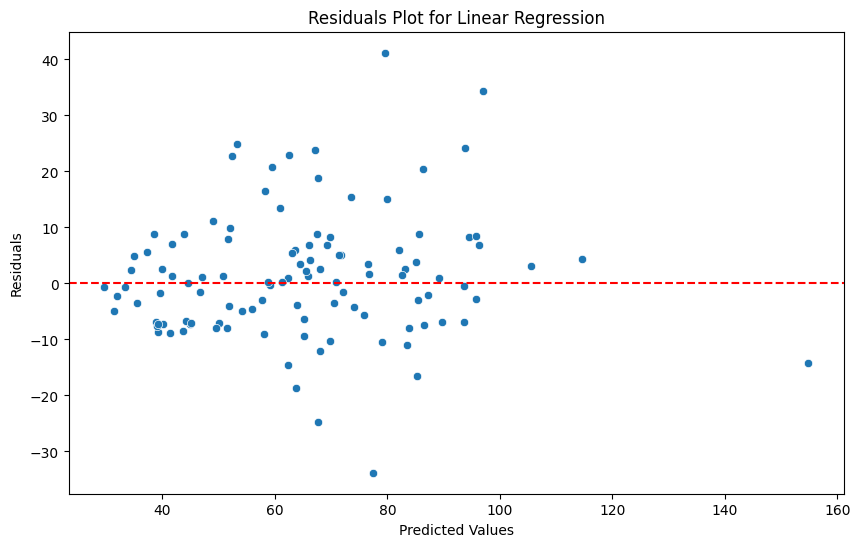
\includegraphics[width=1\linewidth]{images/residuals linear regression.png}
    \caption{Wykres reszt dla Linear Regression}
\end{figure}
\begin{figure}[H]
    \centering
    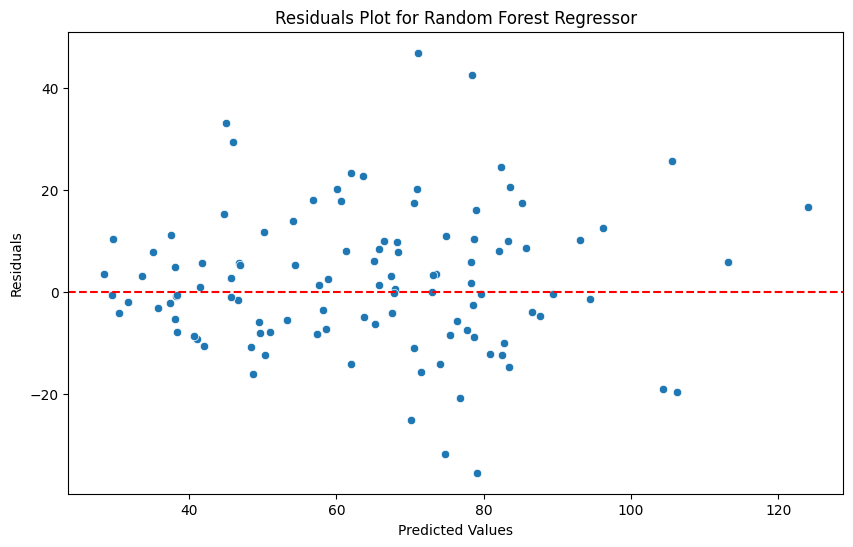
\includegraphics[width=1\linewidth]{images/residuals random forest.png}
    \caption{Wykres reszt dla Random Forest Regressor}
\end{figure}
\begin{figure}[H]
    \centering
    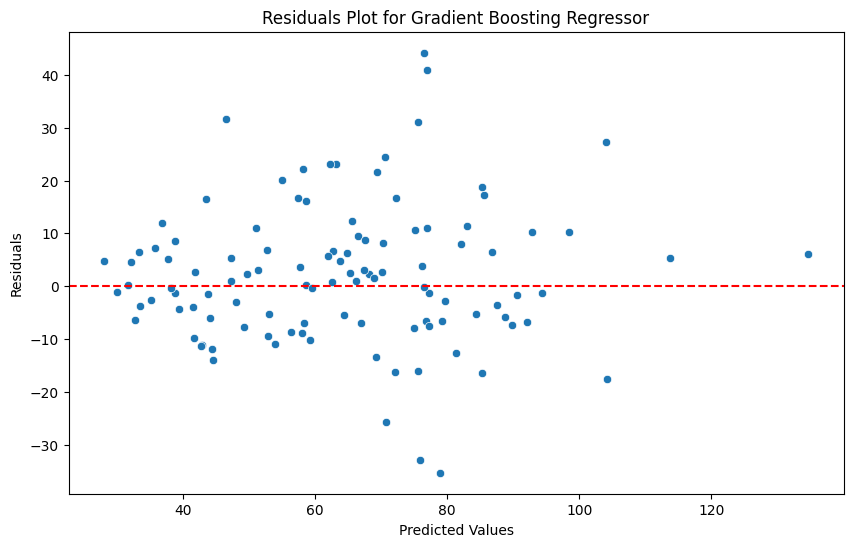
\includegraphics[width=1\linewidth]{images/residuals gradient boosting.png}
    \caption{Wykres reszt dla Gradient Boosting Regressor}
\end{figure}

Wykresy reszt (residuals plot) są dość podobne dla wszystkich modeli. Są jednak pewne różnice. Wygląda na to, że wartości przewidywane metodą Linear Regression są niższe, niż w przypadku innych modeli.

\subsection{Wyniki}

\begin{table}[H]
    \centering
    \caption{Wyniki różnych modeli regresji}
    \label{tab:model_results}
    \begin{tabular}{lccc}
        \toprule
        \textbf{Model} & \textbf{MSE} & \textbf{MAE} & \textbf{R\textsuperscript{2}} \\
        \midrule
        Linear Regression & 126.615 & 8.188 & 0.788 \\
        Random Forest Regressor & 165.674 & 9.947 & 0.722 \\
        Gradient Boosting Regressor & 149.676 & 9.320 & 0.749 \\
        \bottomrule
    \end{tabular}
\end{table}

\begin{table}[H]
    \centering
    \caption{Wyniki różnych modeli regresji na zbiorach testowych i treningowych}
    \begin{tabular}{lcc}
        \toprule
        \textbf{Model} & \textbf{R\textsuperscript{2} (Test)} & \textbf{R\textsuperscript{2} (Train)} \\
        \midrule
        Linear Regression & 0.788 & 0.833 \\
        Random Forest Regressor & 0.722 & 0.939 \\
        Gradient Boosting Regressor & 0.749 & 0.918 \\
        \bottomrule
    \end{tabular}
\end{table}

\subsection{Wnioski}
Najwyższy wynik wśród wartości testowych osiąnął model Linear Regression. Modele Random Forest Regressor i Gradient Boosting Regressor osiągnęły bardzo wysokie wyniki dla danych treningowych, ale zauważalnie niższe dla danych testowych, co sugeruje wystąpienie zjawiska overfitting. Wynik zoptymalizowanego modelu Linear Regression jest praktycznie taki sam, jak w \ref{tab:genetic_metrics}. Wyniki zbliżone do 0,8 można określić jako dobre, biorąc pod uwagę losowość i złożoność symulacji.

\subsection{Uwzględnienie wszystkich parametrów początkowych}
Na koniec został przeprowadzony dodatkowy eksperyment. Jak na wyniki estymacji wpłynęłoby uwzględnienie wszystkich parametrów początkowych? Oto wyniki:
\begin{table}[H]
    \centering
    \caption{Wyniki różnych modeli regresji na zbiorach testowych i treningowych z uwzględnieniem wszystkich parametrów początkowych.}
    \begin{tabular}{lcc}
        \toprule
        \textbf{Model} & \textbf{R\textsuperscript{2} (Test)} & \textbf{R\textsuperscript{2} (Train)} \\
        \midrule
        Linear Regression & 0.818 & 0.879 \\
        Random Forest Regressor & 0.751 & 0.841 \\
        Gradient Boosting Regressor & 0.811 & 0.987 \\
        \bottomrule
    \end{tabular}
\end{table}

Gradient Boosting Regressor doświadczył mocnego overfittingu. Ale zarówno ten model, jak i Linear Regression osiągnęły wyższe wyniki R\textsuperscript{2} dla danych testowych, niż z uwzględnieniem tylko wybranych parametrów początkowych. Wyniki są zauważalnie wyższe.

\section{Wnioski ogólne}
Oczywistym wnioskiem jest to, że dużą częścią niezłych wyników estymacji były parametry początkowe "mnożnik kosztu genów" i "mnożnik kosztu części ciała". Są to parametry, które mogły w złożony sposób wpłynąć na symulację, wprowadzając nieoczekiwane zależności. Stało się tak tylko w części, a zależności między tymi parametrami a średnim kosztem komórki były dość silne i dość liniowe. Na pewno ciekawym eksperymentem byłoby przeprowadzenie analizy jeszcze raz, ale utrzymując obe te parametry jako stałe. 

Kolejnym problemem mógł być zbyt krótki czas symulacji. Prawdopodobnie przy dłuższym czasie symulacji wyniki mogłyby być interesujące. Ilość przeprowadzonych symulacji wydaje się dość adekwatna - overfitting występuje, ale w większości przypadków nie jest bardzo silny.

Ta analiza na pewno pomogłaby podczas rozwoju gry i mogłaby być świetnym narzędziem do optymalizacji parametrów wewnątrz kodu.
\newpage
\bibliographystyle{plain}
\bibliography{references}

\end{document}
